%%%%%%%%%%%%%%%%%%%%%%%%%%%%% Define Article %%%%%%%%%%%%%%%%%%%%%%%%%%%%%%%%%%
\documentclass{article}
%%%%%%%%%%%%%%%%%%%%%%%%%%%%%%%%%%%%%%%%%%%%%%%%%%%%%%%%%%%%%%%%%%%%%%%%%%%%%%%

%%%%%%%%%%%%%%%%%%%%%%%%%%%%% Using Packages %%%%%%%%%%%%%%%%%%%%%%%%%%%%%%%%%%
\usepackage{geometry}
\usepackage{graphicx}
\usepackage{amssymb}
\usepackage{amsmath}
\usepackage{amsthm}
\usepackage{empheq}
\usepackage{mdframed}
\usepackage{booktabs}
\usepackage{lipsum}
\usepackage{graphicx}
\usepackage{color}
\usepackage{psfrag}
\usepackage{pgfplots}
\usepackage{bm}
\usepackage{float}
\usepackage{listings}
\lstset{showstringspaces=false}
%%%%%%%%%%%%%%%%%%%%%%%%%%%%%%%%%%%%%%%%%%%%%%%%%%%%%%%%%%%%%%%%%%%%%%%%%%%%%%%

\date{}

%%%%%%%%%%%%%%%%%%%%%%%%%% Page Setting %%%%%%%%%%%%%%%%%%%%%%%%%%%%%%%%%%%%%%%
\geometry{a4paper}

%%%%%%%%%%%%%%%%%%%%%%%%%% Define some useful colors %%%%%%%%%%%%%%%%%%%%%%%%%%
\definecolor{ocre}{RGB}{243,102,25}
\definecolor{mygray}{RGB}{243,243,244}
\definecolor{deepGreen}{RGB}{26,111,0}
\definecolor{shallowGreen}{RGB}{235,255,255}
\definecolor{deepBlue}{RGB}{61,124,222}
\definecolor{shallowBlue}{RGB}{235,249,255}
%%%%%%%%%%%%%%%%%%%%%%%%%%%%%%%%%%%%%%%%%%%%%%%%%%%%%%%%%%%%%%%%%%%%%%%%%%%%%%%

%%%%%%%%%%%%%%%%%%%%%%%%%% Define an orangebox command %%%%%%%%%%%%%%%%%%%%%%%%
\newcommand\orangebox[1]{\fcolorbox{ocre}{mygray}{\hspace{1em}#1\hspace{1em}}}
%%%%%%%%%%%%%%%%%%%%%%%%%%%%%%%%%%%%%%%%%%%%%%%%%%%%%%%%%%%%%%%%%%%%%%%%%%%%%%%

%%%%%%%%%%%%%%%%%%%%%%%%%%%% English Environments %%%%%%%%%%%%%%%%%%%%%%%%%%%%%
\newtheoremstyle{mytheoremstyle}{3pt}{3pt}{\normalfont}{0cm}{\rmfamily\bfseries}{}{1em}{{\color{black}\thmname{#1}~\thmnumber{#2}}\thmnote{\,--\,#3}}
\newtheoremstyle{myproblemstyle}{3pt}{3pt}{\normalfont}{0cm}{\rmfamily\bfseries}{}{1em}{{\color{black}\thmname{#1}~\thmnumber{#2}}\thmnote{\,--\,#3}}
\theoremstyle{mytheoremstyle}
\newmdtheoremenv[linewidth=1pt,backgroundcolor=shallowGreen,linecolor=deepGreen,leftmargin=0pt,innerleftmargin=20pt,innerrightmargin=20pt,]{theorem}{Theorem}[section]
\theoremstyle{mytheoremstyle}
\newmdtheoremenv[linewidth=1pt,backgroundcolor=shallowBlue,linecolor=deepBlue,leftmargin=0pt,innerleftmargin=20pt,innerrightmargin=20pt,]{definition}{Definition}[section]
\theoremstyle{myproblemstyle}
\newmdtheoremenv[linecolor=black,leftmargin=0pt,innerleftmargin=10pt,innerrightmargin=10pt,]{problem}{Problem}[section]
%%%%%%%%%%%%%%%%%%%%%%%%%%%%%%%%%%%%%%%%%%%%%%%%%%%%%%%%%%%%%%%%%%%%%%%%%%%%%%%

%%%%%%%%%%%%%%%%%%%%%%%%%%%%%%% Plotting Settings %%%%%%%%%%%%%%%%%%%%%%%%%%%%%
\usepgfplotslibrary{colorbrewer}
\pgfplotsset{width=8cm,compat=1.9}
%%%%%%%%%%%%%%%%%%%%%%%%%%%%%%%%%%%%%%%%%%%%%%%%%%%%%%%%%%%%%%%%%%%%%%%%%%%%%%%

%%%%%%%%%%%%%%%%%%%%%%%%%%%%%%% Title & Author %%%%%%%%%%%%%%%%%%%%%%%%%%%%%%%%
\title{IBM Machine Learning Professional Certificate}
\author{Notes by Aheer Srabon}
%%%%%%%%%%%%%%%%%%%%%%%%%%%%%%%%%%%%%%%%%%%%%%%%%%%%%%%%%%%%%%%%%%%%%%%%%%%%%%%

\begin{document}
    \maketitle
    \section{Exploratory Data Analysis for Machine Learning}
    \subsection{Introduction to Artificial Intelligence and Machine Learning}

    \noindent Deep learning (DL) is a subset of machine learning (ML),
    which, in turn, is a subset of artificial intelligence (AI). Two of the
    AI breakthroughs as,
    \begin{itemize}
    	\item Image classification
	\item Machine translation
    \end{itemize}

    \begin{figure}[htp]
	\centering
	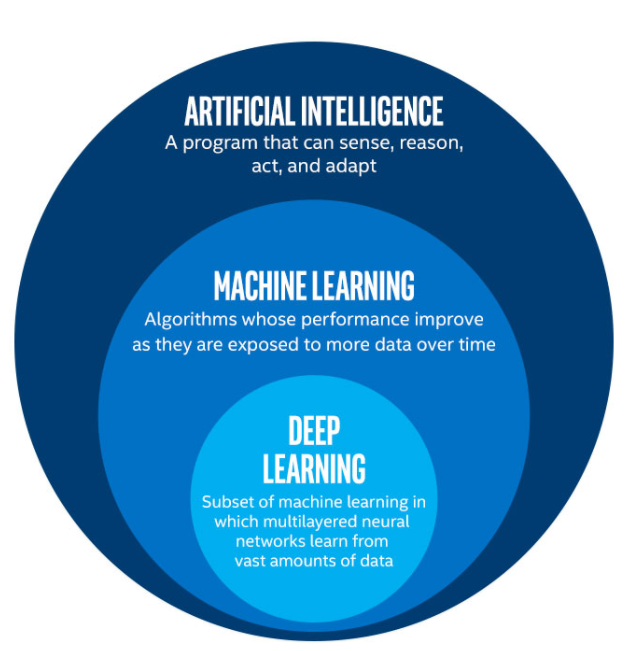
\includegraphics[width=0.25\textwidth]{../assets/AI_ML_DL.png}
    	\caption{Figure 1: AI vs ML vs DL}\label{fig:1}
    \end{figure}

    \subsection{Retrieving and cleaning data}
    \noindent In Python, CSV files can be read by the following command,

    \begin{lstlisting}[language=Python]
    import pandas as pd
    filepath = `data/irish_data.csv'

    # import the data
    data = pd.read_csv(filepath)

    # print a few rows
    print(data.iloc[:5])
    \end{lstlisting}

    \vspace{1cm}

    \noindent Reading CSV files: useful arguments
    \begin{lstlisting}[language=Python]
    # for tab-separated file (.tsv)
    data = pd.read_csv(filepath, sep='\t')

    # space-separated file
    data = pd.read_csv(filepath, delim_whitespace=True)

    # don't use the first row for column names:
    data = pd.read_csv(filepath, header=None)

    # specify column names
    data = pd.read_csv(filepath, names=['Name1', 'Name2'])

    # custom missing values
    data = pd.read_csv(filepath, na_values=['NA', 99])
    \end{lstlisting}

    \vspace{1cm}

    \noindent Reading and writing JSON files,
    \begin{lstlisting}[language=Python]
    # read JSON file as dataframe
    data = pd.read_json(filepath)

    # write dataframe file to JSON
    data = pd.to_json(`outputfile.json')
    \end{lstlisting}

    \vspace{1cm}

    \noindent Reading SQL data,
    \begin{lstlisting}[language=Python]
    import sqlite3 as sq3
    import pandas.io.sql as pds

    # path to SQLite database
    path = `data/classic_rock.db'

    # create connection to SQL database
    con = sq3.Connection(path)

    # write query
    query = ''' SELECT * FROM rock_songs; '''

    # execute query
    data = pds.read_sql(query, con)
    \end{lstlisting}

    \vspace{1cm}

    \noindent The function read\_sql takes in a query to execute, and a
    connection through which it should execute. As long as these two
    are available, it can execute any query through any connection. If
    chunksize argument is passed to read\_sql, it returns a generator
    object which can be iterated. This method helps particularly when the
    dataset is too large to be loaded into the memory of the computer executing
    the script.

    \pagebreak

    \noindent NoSQL databases,
    \begin{itemize}
    	\item Document databases: mongoDB, couchDB
	\item Key-value stores: Riak, Voldemort, Redis
	\item Graph databases: Neo4j, HyperGraph
	\item Wide-column stores: Cassandra, HBase
    \end{itemize}

    \noindent Reading NoSQL data,
    \begin{lstlisting}[language=Python]
    from pymongo import MongoClient

    # create a mongo connection
    con = MongoClient('path/to/or/url/of/mongo/library')

    # choose database (con.list_database_names() will display available
    # databases)
    db = con.database_name

    # create a curson object using a query
    curson = db.collection_name.find(query)

    # expand cursor and construct DataFrame
    df = pd.DataFrame(list(cursor))
    \end{lstlisting}

    \noindent Decisions and analytics are increasingly driven by data and
    models. Key aspects of machine learning workflow depend on cleaned
    data,
    \begin{itemize}
    \itemsep0em
	    \item \textbf{Observations: } An instance of the data 
		    (usually a point or row in a dataset)
	    \item \textbf{Labels: } Output variable(s) being predicted
	    \item \textbf{Algorithms: } Computer programs that estimate
		    models based on available data
	    \item \textbf{Features: } Information we have for each
		    oveservation (variables)
	    \item \textbf{Model: } Hypothesized relationship between
		    observations and data
    \end{itemize}
    \noindent Messy data can lead to "garbage-in, garbage-out" effect,
    and unreliable outcome. The main data problems companies face,
    \begin{itemize}
    	\item Lack of data
	\item Too much data
	\item Bad data
    \end{itemize}

    \noindent Data can be messy,
    \begin{itemize}
    	\item Duplicate or unnecessary data
	\item Inconsistent text and typos
	\item Missing data
	\item Outliers
	\item Data sourcing issues
    \end{itemize}

    \noindent Policies for missing data,
    \begin{itemize}
    	\item \textbf{Remove} the data: remove the row(s) entirely
	\item \textbf{Impute} the data: replace with substituted values
		Fill in the missing data with the most common value,
		the average value, etc
	\item \textbf{Mask} the data: create a category for missing 
		values
    \end{itemize}

    \noindent An \textbf{outlier} is an observation in data that 
    is distant from most other observations. Typically, these observations
    are aberrations and do not accurately represent the phenomenon we
    are trying to explain through the model. Some outliers are important.

    \vspace{1cm}

    \noindent \textbf{Detecting outliers:} using statistics
    \begin{lstlisting}[language=Python]
    import numpy as np

    # calculate the inter-quartile range
    q25, q50, q75 = np.percentile(data, [25, 50, 75])
    iqr = q75 - q25

    # calculate the min and max limits to be considered an outlier
    min = q25 - 1.5*iqr
    max = q75 + 1.5*iqr

    print(min, q25, q50, q75, max)

    # identify the points
    print([x for x in data if x > max])

    # here data is a numpy array
    \end{lstlisting}

    \vspace{1cm}

    \noindent \textbf{Detecting outliers:} using residuals
    \noindent \textbf{Residuals} (difference between actual and predicted
    values of the outcome variable) represent model failure.

    \noindent Approaches to calculating residuals:
    \begin{itemize}
    	\item \textbf{Standardized: } residual divided by standard error
	\item \textbf{Deleted: } residual from fitting model on all data
		excluding current observation
	\item \textbf{Studentized: } deleted residuals divided by residual
		standard error (based on all data, or all data excluding
		    current observation)
    \end{itemize}

    \pagebreak

    \noindent Policies for outliers,
    \begin{itemize}
    	\item Remove
	\item Assign the mean or median
	\item Transform the variable
	\item Predict using regression or some other technique
	\item Keep them, but focus on models that are resistant
		to outliers
    \end{itemize}
    
\end{document}
